\documentclass[10pt,a4paper,UTF8]{article}
\usepackage{zclorg}
\author{张朝龙}
\date{}
\title{有限维向量空间}
\hypersetup{
 pdfauthor={张朝龙},
 pdftitle={有限维向量空间},
 pdfkeywords={},
 pdfsubject={},
 pdfcreator={Emacs 25.0.50.1 (Org mode 8.3.4)}, 
 pdflang={English}}
\begin{document}

\maketitle
\tableofcontents
\titlepic{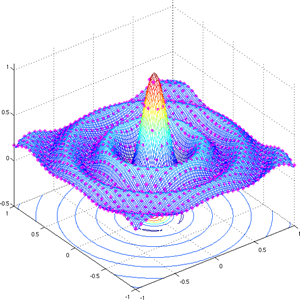
\includegraphics[scale=0.25]{../../img/sinc.PNG}}
\newpage

本文是学习有限维向量空间的笔记,主要内容涉及生成空间,线性无关组,基和维数。



\section{生成空间}
\label{sec:orgheadline1}


\begin{definition}
\(V\)中一组向量\(v_{1},\ldots ,v_{m}\)的所有线性组合构成的集合成为\(v_{1},\ldots ,v_{m}\)的生成空间,记为\(span (v_{1},\ldots ,v_{m})\),即:\[span(v_{1},\ldots ,v_{m})= \{a_{1}v_{1} + \ldots + a_{m}v_{m}: a_{1},\ldots ,a_{m} \in \mathbf{F}\}\]
\end{definition}

\begin{theorem}
定理:生成空间是包含这组向量的最小子空间
\end{theorem}

\begin{proof}
证明:设\(v_{1},\ldots ,v_{m}\) 是\(V\)中的一组向量。先证明: \(span(v_{1},\ldots ,v_{m})\)是\(V\)的子空间(通过证明\(0\)元,加法封闭性,标量乘法封闭性即可证明子空间合理)。加法单位元属于\(span(v_{1},\ldots ,v_{m})\),因为\[0 = 0v_{1} + \ldots + 0v_{m}\]其次,\(span(v_{1},\ldots ,v_{m})\)在加法下封闭,因为:\[(a_{1}v_{1} + \ldots + a_{m}v_{m}) + (c_{1}v_{1} + \ldots + c_{m}v_{m}) = (a_{1} + c_{1})v_{1} + \ldots + (a_{m}+c_{m})v_{m}\]第三,\(span(v_{1},\ldots ,v_{m})\)在标量乘法下封闭,因为:\[\lambda (a_{1}v_{1} + \ldots + a_{m}v_{m}) = \lambda a_{1}v_{1} + \ldots + \lambda a_{m}v_{m}\]

于是:\(span(v_{1},\ldots ,v_{m})\)是\(V\)的子空间。

每个\(v_{j}\)都是\(v_{1},\ldots ,v_{m}\)的线性组合,于是\(span(v_{1},\ldots ,v_{m})\)包含每一个\(v_{j}\)。反之,由于子空间对加法和标量乘法都封闭,从而\(V\)的包含所有\(v_{j}\)的子空间必定\(span(v_{1},\ldots ,v_{m})\)。因此\(span(v_{1},\ldots ,v_{m})\)是\(V\)的包含所有\(v_{1},\ldots ,v_{m}\)的最小子空间。
\end{proof}

\begin{definition}[有限维向量空间]
如果一个向量空间可以由该空间中的某个向量组生成,则称这个向量空间是有限维的。
\end{definition}

\begin{definition}[多项式\(\mathcal{P}(\mathbf{F})\)]
对于函数\(p: \mathbf{F} \rightarrow \mathbf{F}\),若存在\(a_{0},\ldots ,a_{m}\in \mathbf{F}\)使得对任意的\(z\in \mathbf{F}\)均有:\[p(z) = a_{0} + a_{1}z + \ldots + a_{m}z^{m}\]则称\(p\)为系数属于\(\mathbf{F}\)的多项式。

\(\mathcal{P}(\mathbf{F})\)是系数属于\(\mathbf{F}\)的全体多项式所组成的集合。
\end{definition}

在通常的加法和标量乘法下,\(\mathcal{P}(\mathbf{F})\)是\(\mathbf{F}\)上的向量空间,也就是说,\(\mathcal{P}(\mathbf{F})\)是\(\mathbf{F}^{\mathbf{F}}\)(\(\mathbf{F}\)到\(\mathbf{F}\)的全体函数构成的向量空间)的子空间。

如果一个多项式(视为\(\mathbf{F}\)到\(\mathbf{F}\)的函数)可用两组系数来表示,将这两个表达式相减得到一个多项式,该多项式作为\(\mathbf{F}\)上的函数是恒等于零的函数,因此该多项式的系数均为\(0\)。一个多现实的系数由该多项式唯一确定。

\begin{definition}[多项式的次数]
对于多项式\(p\in \mathcal{P}(\mathbf{F})\),若存在标量\(a_{0},a_{1},\ldots ,a_{m}\in \mathbf{F}\),其中\(a_{m}\neq 0\)使得对任意的\(z\in \mathbf{F}\)有\[p(z) = a_{0} + a_{1}z + \ldots + a_{m}z^{m}\]则说\(p\)的次数为\(m\),记为\(deg(p) = m\)

规定恒等于0的多项式次数为\(-\infty\)
\end{definition}

\begin{definition}[\(\mathcal{P}(\mathbf{F})\)]
对于非负整数\(m\),用\(\mathcal{P}_{m}(\mathbf{F})\)表示系数在\(\mathbf{F}\)中且次数不超过\(m\)的所有多项式构成的集合。
\end{definition}
显然:\(\mathcal{P}_{m}(\mathbf{F}) = span(1,z,\ldots ,z^{m})\),对于每个非负整数\(m\),\(\mathcal{P}_{m}(\mathbf{F})\)是有限维向量空间。如果一个向量空间不是有限维的,则成为无限维的。比如\(\mathcal{P}(\mathbf{F})\)就是无限维的。


\begin{theorem}
\(\mathcal{P}(\mathbf{F})\)是无限维的。
\end{theorem}
\begin{proof}
考虑\(\mathcal{P}(\mathbf{F})\)中任意一组元素,记\(m\)是这组多项式的最高次数。则这个组的张成空间中的每个多项式的次数最多为\(m\)。因此\(z^{m+1}\)不属于这个组的张成空间。从而没有组能够张成\(\mathcal{P}(\mathbf{F})\).所以\(\mathcal{P}(\mathbf{F})\)是无限维的。
\end{proof}

\section{线性无关}
\label{sec:orgheadline2}


设\(v_{1},\ldots ,v_{m}\in V\),且\(v\in span(v_{1},\ldots ,v_{m})\),则:\[v = a_{1}v_{1} + \ldots + a_{m}v_{m}\]现在我们来考虑上式中的系数取值是否唯一的问题。假设\(v\)还可以表示为:\[v = c_{1}v_{1} + \ldots + c_{m}v_{m}\]两式相减得到:\[0 = (a_{1}-c_{1})v_{1} + \ldots + (a_{m}-c_{m})v_{m}\]于是我们把\(0\)写成了\(v_{1},\ldots ,v_{m}\)的线性组合,如果\(0\)只能写成每个标量都取零的线性组合,则每个\(a_{i}-c_{i}\)都等于零,即\(a_{i} = c_{i}\)。则我们称\(v_{1},\ldots ,v_{m}\)是线性无关的。

线性无关的一个严格的定义为:
\begin{definition}[线性无关]
\(V\)中的一组向量\(v_{1},\ldots ,v_{m}\)是线性无关的,如果\(a_{1}v_{1} + \ldots + a_{m}v_{m} =0\)的\(a_{1},\ldots ,a_{m}\in \mathbf{F}\)只有\(a_{1} = \ldots = a_{m} = 0\)
\end{definition}

显然, \(a_{1}v_{1} + \ldots + a_{m}v_{m}\)是线性无关的当且仅当\(span(v_{1},\ldots ,v_{m})\)中的每个向量都可以唯一的表示成\(v_{1},\ldots ,v_{m}\)的线性组合。

\begin{instance}
\begin{enumerate}
\item \(V\)中一个向量\(v\)是线性无关的当且仅当\(v\neq 0\)
\item \(V\)中两个向量构成的向量组线性无关当且仅当每个向量都不可以写成另一个向量组的标量倍。
\item \(\mathbf{F}^{4}\)中\((1,0,0,0),(0,1,0,0),(0,0,1,0)\)线性无关
\item 对每个非负整数\(m\), \(\mathcal{P}(\mathbf{F})\)中的组\(1,z,\ldots ,z^{m}\)线性无关
\end{enumerate}
\end{instance}

\begin{definition}[线性相关]
\(V\)中一组向量如果不是线性无关的,则称为线性相关的。也就是说\(V\)中一组向量\(v_{1},\ldots ,v_{m}\)线性相关当且仅当存在不全为零的\(a_{1},\ldots ,a_{m} \in \mathbf{F}\)使得 \(a_{1}v_{1} + \ldots + a_{m}v_{m} = 0\)
\end{definition}

\begin{theorem}[线性相关性引理]
设\(v_{1},\ldots ,v_{m}\)是\(V\)中的一个线性相关的向量组.则有\(j\in \{1,2,\ldots ,m\}\)使得:
\begin{enumerate}
\item \(v_{j} \in span(v_{1},\ldots ,v_{m})\)
\item 若从\(v_{1},\ldots ,v_{m}\)中去掉第\(j\)想,则剩余组的张成空间等于\(span(v_{1},\ldots ,v_{m})\)
\end{enumerate}
\end{theorem}
\begin{proof}
由于向量组\(v_{1},\ldots ,v_{m}\)线性相关,存在不全为\(0\)的\(a_{1},\ldots ,a_{m} \in \mathbf{F}\)使得 \(a_{1}v_{1} + \ldots + a_{m}v_{m} = 0\) ,设\(j\)是\(\{1,\ldots,m\}\)中使得\(a_{j}\neq 0\)的最大者,则:
\begin{equation}
\label{eq:1}
v_{j} = -\frac{a_{1}}{a_{j}} v_{1} - \ldots  - \frac{a_{m}}{a_{j}}v_{m}
\end{equation}
接下来,我们证明第二步,设\(u\in span(v_{1},\ldots ,v_{m})\),则存在\(c_{1},\ldots ,c_{m} \in \mathbf{F}\)使得:\[u = c_{1}v_{1} + \ldots + c_{m}v_{m}\] 带入\ref{eq:1},可得\(u\)属于从\(v_{1},\ldots ,v_{m}\)中去掉第\(j\)项所得到的组的张成空间。
\end{proof}

接下来我们看一个重要的结论:
\begin{theorem}
在有限维向量空间中,线性无关组中向量的个数不超过向量空间的每个张成组的向量个数。
\end{theorem}

\begin{proof}
设\(u_{1},\ldots,u_{m}\)在\(V\)中是线性无关的,并设\(w_{1},\ldots ,w_{n}\)张成\(V\),我们需要证明\(m \leq n\)。

设\(B\)表示\(V\)的张成组\(w_{1},\ldots ,w_{n}\).在该组上添加任何向量都会得到一个线性相关组,特别的,组\[u_{1},w_{1},\ldots ,w_{n}\]是线性相关的,那么可以通过去掉某个\(w\)使得\(u_{1}\)和余下的\(w\)构成新的\(B\),这个\(B\)同样张成\(V\)。

依次类推,假设我们执行了到了第 \(j\)步,我们知道经过前\(j-1\)步生成的\(B\)张成了\(V\),从而再添加任何向量都会构成线性相关组,特别的我们在\(u_{1},\ldots ,u_{j-1}\)之后添加\(u_{j}\),\(u_{1},\ldots ,u_{j}\)和之前剩下的\(w\)构成了\(n+1\)个向量组,所以是线性相关的,此时我们需要从\(n+1\)个向量组中减去一个,又因为\(u_{1},\ldots ,u_{j}\)是线性无关的,所以这个向量一定是某个\(w\),而不是某个\(u\),我们可以从\(B\)中去掉这个\(w\),那么新的\(B\)仍然张成\(V\)

经过\(m\)步之后,新的\(B\)由\(u_{1},\ldots ,u_{m}\)和剩下的\(w\)一起构成。因此\(w\)的个数至少和\(u\)的个数一样多。
\end{proof}

关于这个结论的直接应用,我们给两个例子。
\begin{instance}
证明组\((1,2,3),(4,5,8),(9,6,7),(-3,2,8)\)在\(\mathbf{R}^{3}\)中不是线性无关组。

因为组\((1,0,0),(0,1,0),(0,0,1)\)张成了\(\mathbf{R}^{3}\)。所以在\(\mathbf{R}^{3}\)中不可能存在向量个数大于3的线性无关组。
\end{instance}

\begin{instance}
证明组\((1,2,3,-5),(4,5,8,3),(9,6,7,-1)\)不能张成\(\mathbf{R}^{4}\)

因为\((1,0,0,0),(0,1,0,0),(0,0,1,0),(0,0,0,1)\)在\(\mathbf{R}^{4}\)中是线性无关的,所以个数为4的组不能张成\(\mathbf{R}^{4}\). 线性无关组中向量的个数不超过向量空间的每个张成组的向量个数。
\end{instance}

\begin{theorem}
有限维向量空间的子空间都是有限维的
\end{theorem}
\begin{proof}
设\(V\)是有限维向量空间,\(U\)是\(V\)的子空间,只需要证明\(U\)是有限维的。我们通过以下步骤来证明:

\begin{enumerate}
\item 若\(U={0}\),则\(U\)是有限维的,得证。若\(U\neq {0}\)则取非零向量\(v_{1}\in U\)
\item 若\(U = span(v_{1},\ldots ,v_{j-1})\),则\(U\)是有限维的,得证。若\(U \neq span(v_{1},\ldots ,v_{j-1})\) 则取一个向量\(v_{j}\in U\)使得\(v_{j} \notin span(v_{1},\ldots ,v_{j-1})\) 经过每一步,只要这个程序还在继续,我们都构造了一个向量组,其中每一个新添加的向量都不在它前面的张成空间中,因此每一步我们都构成了一个线性无关组。另外,我们知道这个线性无关组不能比\(V\)的任何张成组中的向量个数还大。这个构建过程一定会终止,因此,\(U\)是有限维的。
\end{enumerate}
\end{proof}

\section{基}
\label{sec:orgheadline3}


接下来,我们搞基。
\begin{definition}[基]
若\(V\)中一个向量组既线性无关又张成\(V\),则称这个线性无关组为\(V\)的基
\end{definition}

\begin{instance}
\begin{enumerate}
\item 组\((1,0,0,\ldots ,0),(0,1,0,\ldots ,0),\ldots ,(0,\ldots ,0,1)\) 是\(\mathbf{F}^{n}\)的基,称为\(\mathbf{F}^{n}\)的标准基
\item 组\((1,2),(3,5)\)是\(\mathbf{F}^{2}\)的基
\item 组\((1,2,-4),(7,-5,6)\)在\(\mathbf{F}^{3}\)中线性无关,但不是\(\mathbf{F}^{3}\)的基,因为不能张成\(\mathbf{F}^{3}\)
\item 组\((1,2),(3,5),(4,13)\)张成\(\mathbf{F}^{2}\)但不是\(\mathbf{F}^{2}\)的基,因为它不是线性无关的。
\item 组\((1,1,0),(0,0,1)\)是\(\{(x,x,y)\in \mathbf{F}^{3}:x,y\in \mathbf{F}\}\)的基。
\item 组\((1,-1,0),(1,0,-1)\)是\(\{(x,y,z)\in \mathbf{F}^{3}:x + y + z = 0\}\)的基。
\item 组\(1,z,\ldots ,z^{m}\)是\(\mathcal{P}_{m}(\mathbf{F})\)的基
\end{enumerate}
\end{instance}

\begin{theorem}[基的判定准则]
\(V\)中的向量组\(v_{1},\ldots ,v_{n}\)是\(V\)的基,当且仅当每个\(v\in V\)都能唯一的写成:\[v  = a_{1}v_{1} + \ldots + a_{n}v_{n}\]其中\(a_{1},\ldots ,a_{n}\in \mathbf{F}\)
\end{theorem}
\begin{proof}
设\(v_{1},\ldots ,v_{n}\)是\(V\)的基,并设\(v\in V\),因此\(v\)可以写成\[v  = a_{1}v_{1} + \ldots + a_{n}v_{n}\],假设\(v\)还可以写成\[v  = c_{1}v_{1} + \ldots + c_{n}v_{n}\]两式相减,得:
\[0  = (a_{1}- c_{1})v_{1} + \ldots + (a_{n}-c_{n})v_{n}\]由于\(v_{1},\ldots ,v_{n}\)是线性无关的,所以每个\(a_{j} - c_{j}=0\),因此\(a_{1} = c_{1},\ldots ,a_{n} = c_{n}\),这就证明了唯一性。

接下来假设\(v\in V\)可以唯一的写成\[v  = a_{1}v_{1} + \ldots + a_{n}v_{n}\] ,我们来证明\(v_{1},\ldots ,v_{n}\)线性无关。设\(a_{1},\ldots ,a_{n}\in \mathbf{F}\)使得\[0  = a_{1}v_{1} + \ldots + a_{n}v_{n}\],由于表示的唯一性,所以\(a_{1} = \ldots  = a_{n} = 0\),因此\(v_{1},\ldots ,v_{n}\)线性无关。由于\(v_{1},\ldots ,v_{n}\)线性无关又张成了\(V\)所以\(v_{1},\ldots ,v_{n}\)是\(V\)的基。
\end{proof}

向量空间的张成组不一定是基,因为它可能是线性相关的。但是我们总可以去掉其中的某些向量使得这个线性相关组变成线性无关组。
\begin{theorem}[张成组包含基]
在向量空间中,每个张成组都可以简化为一个基
\end{theorem}

\begin{proof}
设\(v_{1},\ldots ,v_{n}\)张成\(V\),我们要从\(v_{1},\ldots ,v_{n}\)中去掉那些多余的向量来构造基。我们用\(B\)来表示\(v_{1},\ldots ,v_{n}\)。

\begin{enumerate}
\item 若\(v_{1} = 0\),则从\(B\)中去掉\(v_{1}\);若\(v_{1} \neq 0\),则保持\(B\)不变。
\item 若\(v_{j}\in span(v_{1},\ldots ,v_{j-1})\),则从\(B\)中去掉\(v_{j}\);否则保持\(B\)不变。
\end{enumerate}

经过\(n\)步以后,终止操作,得到一个向量组。因为最初的向量组张成\(V\),而去掉的向量都可以使用剩下的向量表示,所以剩下的向量组也张成\(V\)。又因为这个过程确保剩下的向量是线性无关的,所以剩下的向量组构成了\(V\)的基。
\end{proof}
显然,从有限维向量空间的定义出发,每个有限维向量空间都有基。更进一步,针对有限维向量空间的线性无关的向量组,我们都可以扩展出一组线性无关组使其构成有限维向量空间的基。

设\(V\)是有限维的,\(u_{1},\ldots ,u_{m}\)在\(V\)中线性无关,设\(w_{1},\ldots ,w_{n}\)是\(V\)的一个基。则向量组\(u_{1},\ldots ,u_{m},w_{1},\ldots ,w_{n}\)张成\(V\)。我们可以把这个向量组通过去掉某些\(w\)变成\(V\)的一个基,这个基包含了所有的\(u\)和某些\(w\)。写到这里,是不是想到了之前直和的概念?那些多出来的\(w\)是什么?这些\(u\)又是什么?

\begin{theorem}[\(V\)的每个子空间都是\(V\)的直和项]
设\(V\)是有限维的,\(U\)是\(V\)的子空间 ,则存在\(V\)的子空间\(W\)使得\(V = U\oplus W\)
\end{theorem}

\begin{proof}
证明: 因为\(V\)是有限维的,所以\(U\)也是有限维,并且\(U\)有一个基\(u_{1},\ldots ,u_{m}\)。\(u_{1},\ldots ,u_{m}\)也是\(V\)中的一个线性无关组,从而可以扩充成\(V\)的一个基,假设扩充后的向量无关组是\(u_{1},\ldots ,u_{m},w_{1},\ldots ,w_{n}\),令\(W = span(w_{1},\ldots ,w_{n})\). 要证明\(V = U \oplus W\), 我们只需要证明\[V = U + W, \{0\} = U \cap W\] 首先,我们证明\(V = U + W\).设\(V\)中一个向量\(v\),可以表示为\[v = \underbrace{a_{1}u_{1} + \ldots +a_{m}u_{m}}_{u} + \underbrace{b_{1}w_{1} \ldots  + b_{n}w_{n}}_{w}\] 显然\(u\in U, w\in W,v = u+w\),因此\(v\in U + W, V = U+ W\).

然后我们证明\(U\cap W = \{0\}\),假设\(v \in U\cap W\),存在\(a_{1},\ldots ,a_{m},b_{1},\ldots ,b_{n} \in \mathbf{F}\)使得:
\[v = a_{1}u_{1} + \ldots + a_{m}u_{m} = b_{1}w_{1} + \ldots + b_{n}w_{n}\]
因此,有:
\[ a_{1}u_{1} + \ldots + a_{m}u_{m} - b_{1}w_{1} - \ldots - b_{n}w_{n} = 0\]
又因为\(u_{1},\ldots ,u_{m},w_{1},\ldots ,w_{n}\)是线性无关组,所以只有\(v=0\),即\(U\cap W = \{0\}\)

综上,命题得证。
\end{proof}
\section{维数}
\label{sec:orgheadline4}


至此我们讨论了有限维线性空间的基,讨论了基的构造过程。我们还需要讨论有限维线性空间的另外一个重要概念:维数。如何定义维数?一个合理的定义应该保证\(\mathbf{F}^{n}\)的维数是\(n\)。因为我们知道\(\mathbf{F}^{n}\)标准基中线性无关组向量的个数是\(n\)。但是对于一个有限维线性空间,其基的个数不止一个,是不是每个基都有相同个数的线性无关向量组呢?是的,我们这就给出证明。

\begin{theorem}[基中线性无关组向量个数不依赖基的选取]
有限维向量空间的任意两个基中线性无关组向量的个数相同
\end{theorem}
\begin{proof}
设\(V\)是有限维的,\(B_{1},B_{2}\)是其任意两个基,则\(B_{1}\)在\(V\)中是线性无关的,并且\(B_{2}\)张成\(V\),通过本文之前我们证明过得结论:有限维线性空间中线性无关组中向量个数不超过基中向量个数。我们知道\(B_{1}\)中向量个数不超过\(B_{2}\)中向量个数。交换\(B_{1}\)和\(B_{2}\)的位置,我们知道\(B_{2}\)中向量个数也不超过\(B_{1}\)中向量个数。因此\(B_{1}\)和\(B_{2}\)中向量个数相同。
\end{proof}
\begin{definition}
有限维向量空间的任意基中线性无关组向量的个数称为这个向量空间的维数;若\(V\)是有限维的,则称\(V\)的维数为\(\dim V\)
\end{definition}
显然,\(\mathbf{F}^{n}\)的维数是\(n\);\(\mathcal{P}_{m}(\mathbf{F})\)的维数是\(m+1\)

要验证\(V\)中的一个向量组是\(V\)的基,按照定义我们必须证明这个向量组满足两个性质:
\begin{enumerate}
\item 这个向量组是线性无关的;
\item 这个向量组张成\(V\)
\end{enumerate}

我们把一个向量组中向量的个数称为这个向量组的长度。

\begin{theorem}
若\(V\)是有限维的,则\(V\)中每个长度为\(\dim V\)的线性无关组都是\(V\)的基。若\(V\)是有限维的,则\(V\)中每个长度为\(\dim V\)的张成组都是\(V\)的基。
\end{theorem}

接下来我们证明一个非常重要的定理:
\begin{theorem}
如果\(U_{1}\)和\(U_{2}\)是有限维向量空间的两个子空间,则\[\dim (U_{1} + U_{2}) = \dim U_{1} + \dim U_{2} -\dim (U_{1}\cap U_{2})\]
\end{theorem}
\begin{proof}
设\(u_{1},\ldots ,u_{m}\)是\(U_{1}\cap U_{2}\)的基,则\(\dim (U_{1}\cap U_{2}) = m\), 又因为\(u_{1},\ldots ,u_{m}\) 是\(U_{1}\)中的线性无关组,则\(u_{1},\ldots ,u_{m}\)可以扩充成\(U_{1}\)的一组基,\(u_{1},\ldots ,u_{m},v_{1},\ldots ,v_{j}\),\(\dim U_{1} = m + j\);同理\(u_{1},\ldots ,u_{m}\)也可以扩充成\(U_{2}\)的一组基,\(u_{1},\ldots ,u_{m},w_{1},\ldots ,w_{k}\) ,\(\dim U_{2} = m + k\),倘若我们能够证明\(u_{1},\ldots ,u_{m},v_{1},\ldots ,v_{j},w_{1},\ldots ,w_{k}\)是\(U_{1} + U_{2}\)的一组基,则我们可以得到:
\begin{eqnarray*}
\dim(U_{1} \cap U_{2}) &= & m + j + k \\
&=& (m+j) + (m+k) -m \\
&=& \dim(U_{1}) + \dim(U_{2}) - \dim(U_{1}\cap U_{2})
\end{eqnarray*}
\end{proof}
显然\(span(u_{1},\ldots ,u_{m},v_{1},\ldots ,v_{j},w_{1},\ldots ,w_{k})\)张成了\(U_{1} + U_{2}\),接下来我们只需要证明\(u_{1},\ldots ,u_{m},v_{1},\ldots ,v_{j},w_{1},\ldots ,w_{k}\)是线性无关的。为此我们假设:
\begin{equation}
\label{eq:2}
a_{1}u_{1} + \ldots +a_{m}u_{m} + b_{1}v_{1} + \ldots + b_{j}v_{j} + c_{1}w_{1} + \ldots + c_{k}w_{k} = 0
\end{equation}

则有:
\begin{equation}
\label{eq:3}
c_{1}w_{1} + \ldots + c_{k}w_{k} = -a_{1}u_{1} - \ldots -a_{m}u_{m} - b_{1}v_{1} - \ldots - b_{j}v_{j}  
\end{equation}
所以\(c_{1}w_{1} + \ldots + c_{k}w_{k}\in U_{1}\),又因为\(w_{i}\in U_{2}\),所以存在\(d_{1},\ldots ,d_{m}\)使得:
\begin{equation}
\label{eq:4}
c_{1}w_{1} + \ldots + c_{k}w_{k} = d_{1}u_{1} + \ldots +d_{m}u_{m}
\end{equation}
即:
\begin{equation}
\label{eq:5}
c_{1}w_{1} + \ldots + c_{k}w_{k} - d_{1}u_{1} - \ldots -d_{m}u_{m} = 0;
\end{equation}
又因为 \(u_{1},\ldots ,u_{m},w_{1},\ldots ,w_{k}\)是线性无关组,所以\(c_{1},\ldots ,c_{k},d_{1},\ldots ,d_{m}\)都是零。根据\ref{eq:3}得,所有的\(a\)和\(b\)都是零。因此根据\ref{eq:2},\(u_{1},\ldots ,u_{m},v_{1},\ldots ,v_{j},w_{1},\ldots ,w_{k}\)是线性无关的。至此,命题得证。
\end{document}
